% !TeX spellcheck = pl_PL
%%%%%%%%%%%%%%%%%%%%%%%%%%%%%%%%%%%%%%%%%%%
%                                        %
% Szablon pracy dyplomowej inzynierskiej %
% zgodny  z aktualnymi  przepisami  SZJK %
%                                        %
%%%%%%%%%%%%%%%%%%%%%%%%%%%%%%%%%%%%%%%%%%
%                                        %
%  (c) Krzysztof Simiński, 2018-2023     %
%                                        %
%%%%%%%%%%%%%%%%%%%%%%%%%%%%%%%%%%%%%%%%%%
%                                        %
% Najnowsza wersja szablonów jest        %
% podstępna pod adresem                  %
% github.com/ksiminski/polsl-aei-theses  %
%                                        %
%%%%%%%%%%%%%%%%%%%%%%%%%%%%%%%%%%%%%%%%%%
%
%
% Projekt LaTeXowy zapewnia odpowiednie formatowanie pracy,
% zgodnie z wymaganiami Systemu zapewniania jakości kształcenia.
% Proszę nie zmieniać ustawień formatowania (np. fontu,
% marginesów, wytłuszczeń, kursywy itd. ).
%
% Projekt można kompilować na kilka sposobów.
%
% 1. kompilacja pdfLaTeX
%
% pdflatex main
% bibtex   main
% pdflatex main
% pdflatex main
%
%
% 2. kompilacja XeLaTeX
%
% Kompilatacja przy użyciu XeLaTeXa różni się tym, że na stronie
% tytułowej używany jest font Calibri. Wymaga to jego uprzedniego
% zainstalowania.
%
% xelatex main
% bibtex  main
% xelatex main
% xelatex main
%
%
%%%%%%%%%%%%%%%%%%%%%%%%%%%%%%%%%%%%%%%%%%%%%%%%%%%%%
% W przypadku pytań, uwag, proszę pisać na adres:   %
%      krzysztof.siminski(małpa)polsl.pl            %
%%%%%%%%%%%%%%%%%%%%%%%%%%%%%%%%%%%%%%%%%%%%%%%%%%%%%
%
% Chcemy ulepszać szablony LaTeXowe prac dyplomowych.
% Wypełniając ankietę spod poniższego adresu pomogą
% Państwo nam to zrobić. Ankieta jest całkowicie
% anonimowa. Dziękujemy!


% https://docs.google.com/forms/d/e/1FAIpQLScyllVxNKzKFHfILDfdbwC-jvT8YL0RSTFs-s27UGw9CKn-fQ/viewform?usp=sf_link
%
%%%%%%%%%%%%%%%%%%%%%%%%%%%%%%%%%%%%%%%%%%%%%%%%%%%%%%%%%%%%%%%%%%%%%%%%%

%%%%%%%%%%%%%%%%%%%%%%%%%%%%%%%%%%%%%%%%%%%%%%%
%                                             %
% PERSONALIZACJA PRACY – DANE PRACY           %
%                                             %
%%%%%%%%%%%%%%%%%%%%%%%%%%%%%%%%%%%%%%%%%%%%%%%

% Proszę wpisać swoje dane w poniższych definicjach.

% TODO
% dane autora
\newcommand{\FirstNameAuthor}{Krzysztof}
\newcommand{\SurnameAuthor}{Grądek}
\newcommand{\IdAuthor}{300362}   % numer albumu  (bez $\langle$ i $\rangle$)

% drugi autor:
%\newcommand{\FirstNameCoauthor}{Imię}   % Jeżeli jest drugi autor, to tutaj należy podać imię.
%\newcommand{\SurnameCoauthor}{Nazwisko} % Jeżeli jest drugi autor, to tutaj należy podać nazwisko.
%\newcommand{\IdCoauthor}{$\langle$wpisać właściwy$\rangle$}  % numer albumu drugiego autora (bez $\langle$ i $\rangle$)
% Gdy nie ma drugiego autora, należy zostawić poniższe definicje puste, jak poniżej. Gdy jest drugi autor, należy zakomentować te linie.
\newcommand{\FirstNameCoauthor}{} % Jeżeli praca ma tylko jednego autora, to dane drugiego autora zostają puste.
\newcommand{\SurnameCoauthor}{}   % Jeżeli praca ma tylko jednego autora, to dane drugiego autora zostają puste.
\newcommand{\IdCoauthor}{}  % Jeżeli praca ma tylko jednego autora, to dane drugiego autora zostają puste.
%%%%%%%%%%

\newcommand{\Supervisor}{dr inż. Krzysztof Jaskot}     % dane promotora (bez $\langle$ i $\rangle$)
\newcommand{\Title}{Budowa mapy otoczenia z wykorzystaniem robota mobilnego}           % tytuł pracy po polsku
\newcommand{\TitleAlt}{Construction of an Environment Map Using a Mobile Robot}                     % thesis title in English
\newcommand{\Program}{Automatyka i Robotyka}            % kierunek studiów  (bez $\langle$ i $\rangle$)
\newcommand{\Specialisation}{Technologie Informacyjne}     % specjalność  (bez $\langle$ i $\rangle$)
\newcommand{\Departament}{Katedra Automatyki i Robotyki}        % katedra promotora  (bez $\langle$ i $\rangle$)

% Jeżeli został wyznaczony promotor pomocniczy lub opiekun, proszę go/ją wpisać ...
%\newcommand{\Consultant}{$\langle$stopień naukowy imię i nazwisko$\rangle$} % dane promotora pomocniczego, opiekuna (bez $\langle$ i $\rangle$)
% ... w przeciwnym razie proszę zostawić puste miejsce jak poniżej:
\newcommand{\Consultant}{} % brak promotowa pomocniczego / opiekuna

% koniec fragmentu do modyfikacji
%%%%%%%%%%%%%%%%%%%%%%%%%%%%%%%%%%%%%%%%%%


%%%%%%%%%%%%%%%%%%%%%%%%%%%%%%%%%%%%%%%%%%%%%%%
%                                             %
% KONIEC PERSONALIZACJI PRACY                 %
%                                             %
%%%%%%%%%%%%%%%%%%%%%%%%%%%%%%%%%%%%%%%%%%%%%%%

%%%%%%%%%%%%%%%%%%%%%%%%%%%%%%%%%%%%%%%%


%%%%%%%%%%%%%%%%%%%%%%%%%%%%%%%%%%%%%%%%%%%%%%%
%                                             %
% PROSZĘ NIE MODYFIKOWAĆ PONIŻSZYCH USTAWIEŃ! %
%                                             %
%%%%%%%%%%%%%%%%%%%%%%%%%%%%%%%%%%%%%%%%%%%%%%%



\documentclass[a4paper,twoside,12pt]{book}
\usepackage[utf8]{inputenc}                                      
\usepackage[T1]{fontenc}  
\usepackage{amsmath,amsfonts,amssymb,amsthm}
\usepackage[british,polish]{babel} 
\usepackage{indentfirst}
\usepackage{xurl}
\usepackage{xstring}
\usepackage{ifthen}



\usepackage{ifxetex}

\ifxetex
	\usepackage{fontspec}
	\defaultfontfeatures{Mapping=tex—text} % to support TeX conventions like ``——-''
	\usepackage{xunicode} % Unicode support for LaTeX character names (accents, European chars, etc)
	\usepackage{xltxtra} % Extra customizations for XeLaTeX
\else
	\usepackage{lmodern}
\fi



\usepackage[margin=2.5cm]{geometry}
\usepackage{graphicx} 
\usepackage{hyperref}
\usepackage{booktabs}
\usepackage{tikz}
\usepackage{pgfplots}
\usepackage{mathtools}
\DeclareMathOperator*{\argmin}{arg\,min}
\usepackage{geometry}
\usepackage{subcaption}   % subfigures
\usepackage[page]{appendix} % toc,
\renewcommand{\appendixtocname}{Dodatki}
\renewcommand{\appendixpagename}{Dodatki}
\renewcommand{\appendixname}{Dodatek}

\usepackage{csquotes}
\usepackage[natbib=true,backend=bibtex,maxbibnames=99]{biblatex}  % kompilacja bibliografii BibTeXem
%\usepackage[natbib=true,backend=biber,maxbibnames=99]{biblatex}  % kompilacja bibliografii Biberem
\bibliography{biblio}

\usepackage{ifmtarg}   % empty commands  

\usepackage{setspace}
\onehalfspacing


\frenchspacing

%%%%%%%%%%%%%%%%%%%%%%%%%%%%%%%%%%
% środowiska dla definicji, twierdzenia, przykładu
\usepackage{amsthm}

\newtheorem{Definition}{Definicja}
\newtheorem{Example}{Przykład}
\newtheorem{Theorem}{Twierdzenie}
%%%%%%%%%%%%%%%%%%%%%%%%%%%%%%%%%%

%%%% TODO LIST GENERATOR %%%%%%%%%

\usepackage{color}
\definecolor{brickred}      {cmyk}{0   , 0.89, 0.94, 0.28}

\makeatletter \newcommand \kslistofremarks{\section*{Uwagi} \@starttoc{rks}}
  \newcommand\l@uwagas[2]
    {\par\noindent \textbf{#2:} %\parbox{10cm}
{#1}\par} \makeatother


\newcommand{\ksremark}[1]{%
{%\marginpar{\textdbend}
{\color{brickred}{[#1]}}}%
\addcontentsline{rks}{uwagas}{\protect{#1}}%
}

\newcommand{\comma}{\ksremark{przecinek}}
\newcommand{\nocomma}{\ksremark{bez przecinka}}
\newcommand{\styl}{\ksremark{styl}}
\newcommand{\ortografia}{\ksremark{ortografia}}
\newcommand{\fleksja}{\ksremark{fleksja}}
\newcommand{\pauza}{\ksremark{pauza `--', nie dywiz `-'}}
\newcommand{\kolokwializm}{\ksremark{kolokwializm}}
\newcommand{\cudzyslowy}{\ksremark{,,polskie cudzysłowy''}}

%%%%%%%%%%%%%% END OF TODO LIST GENERATOR %%%%%%%%%%%

\newcommand{\printCoauthor}{%		
    \StrLen{\FirstNameCoauthor}[\FNCoALen]
    \ifthenelse{\FNCoALen > 0}%
    {%
		{\large\bfseries\Coauthor\par}
	
		{\normalsize\bfseries \LeftId: \IdCoauthor\par}
    }%
    {}
} 

%%%%%%%%%%%%%%%%%%%%%
\newcommand{\autor}{%		
    \StrLen{\FirstNameCoauthor}[\FNCoALenXX]
    \ifthenelse{\FNCoALenXX > 0}%
    {\FirstNameAuthor\ \SurnameAuthor, \FirstNameCoauthor\ \SurnameCoauthor}%
	{\FirstNameAuthor\ \SurnameAuthor}%
}
%%%%%%%%%%%%%%%%%%%%%

\StrLen{\FirstNameCoauthor}[\FNCoALen]
\ifthenelse{\FNCoALen > 0}%
{%
\author{\FirstNameAuthor\ \SurnameAuthor, \FirstNameCoauthor\ \SurnameCoauthor}
}%
{%
\author{\FirstNameAuthor\ \SurnameAuthor}
}%

%%%%%%%%%%%% ZYWA PAGINA %%%%%%%%%%%%%%%
% brak kapitalizacji zywej paginy
\usepackage{fancyhdr}
\pagestyle{fancy}
\fancyhf{}
\fancyhead[LO]{\nouppercase{\it\rightmark}}
\fancyhead[RE]{\nouppercase{\it\leftmark}}
\fancyhead[LE,RO]{\it\thepage}


\fancypagestyle{tylkoNumeryStron}{%
   \fancyhf{} 
   \fancyhead[LE,RO]{\it\thepage}
}

\fancypagestyle{bezNumeracji}{%
   \fancyhf{} 
   \fancyhead[LE,RO]{}
}


\fancypagestyle{NumeryStronNazwyRozdzialow}{%
   \fancyhf{} 
   \fancyhead[LE]{\nouppercase{\autor}}
   \fancyhead[RO]{\nouppercase{\leftmark}} 
   \fancyfoot[CE, CO]{\thepage}
}


%%%%%%%%%%%%% OBCE WTRETY  
\newcommand{\obcy}[1]{\emph{#1}}
\newcommand{\english}[1]{{\selectlanguage{british}\obcy{#1}}}
%%%%%%%%%%%%%%%%%%%%%%%%%%%%%

% polskie oznaczenia funkcji matematycznych
\renewcommand{\tan}{\operatorname {tg}}
\renewcommand{\log}{\operatorname {lg}}

% jeszcze jakies drobiazgi

\newcounter{stronyPozaNumeracja}

%%%%%%%%%%%%%%%%%%%%%%%%%%% 
\newcommand{\printOpiekun}[1]{%		

    \StrLen{\Consultant}[\mystringlen]
    \ifthenelse{\mystringlen > 0}%
    {%
       {\large{\bfseries OPIEKUN, PROMOTOR POMOCNICZY}\par}
       
       {\large{\bfseries \Consultant}\par}
    }%
    {}
} 
%
%%%%%%%%%%%%%%%%%%%%%%%%%%%%%%%%%%%%%%%%%%%%%%
 
% Proszę nie modyfikować poniższych definicji!
\newcommand{\Author}{\FirstNameAuthor\ \MakeUppercase{\SurnameAuthor}} 
\newcommand{\Coauthor}{\FirstNameCoauthor\ \MakeUppercase{\SurnameCoauthor}}
\newcommand{\Type}{PROJEKT INŻYNIERSKI}
\newcommand{\Faculty}{Wydział Automatyki, Elektroniki i Informatyki} 
\newcommand{\Polsl}{Politechnika Śląska}
\newcommand{\Logo}{politechnika_sl_logo_bw_pion_pl.pdf}
\newcommand{\LeftId}{Nr albumu}
\newcommand{\LeftProgram}{Kierunek}
\newcommand{\LeftSpecialisation}{Specjalność}
\newcommand{\LeftSUPERVISOR}{PROWADZĄCY PRACĘ}
\newcommand{\LeftDEPARTMENT}{KATEDRA}
%%%%%%%%%%%%%%%%%%%%%%%%%%%%%%%%%%%%%%%%%%%%%%

%%%%%%%%%%%%%%%%%%%%%%%%%%%%%%%%%%%%%%%%%%%%%%%
%                                             %
% KONIEC USTAWIEŃ                             %
%                                             %
%%%%%%%%%%%%%%%%%%%%%%%%%%%%%%%%%%%%%%%%%%%%%%%




%%%%%%%%%%%%%%%%%%%%%%%%%%%%%%%%%%%%%%%%%%%%%%%
%                                             %
% MOJE PAKIETY, USTAWIENIA ITD                %
%                                             %
%%%%%%%%%%%%%%%%%%%%%%%%%%%%%%%%%%%%%%%%%%%%%%%

% Tutaj proszę umieszczać swoje pakiety, makra, ustawienia itd.


 
%%%%%%%%%%%%%%%%%%%%%%%%%%%%%%%%%%%%%%%%%%%%%%%%%%%%%%%%%%%%%%%%%%%%%
% listingi i fragmentu kodu źródłowego 
% pakiet: listings lub minted
% % % % % % % % % % % % % % % % % % % % % % % % % % % % % % % % % % % 

% biblioteka listings
\usepackage{listings}
\lstset{%
morekeywords={string,exception,std,vector},% słowa kluczowe rozpoznawane przez pakiet listings
language=C++,% C, Matlab, Python, SQL, TeX, XML, bash, ... – vide https://www.ctan.org/pkg/listings
commentstyle=\textit,%
identifierstyle=\textsf,%
keywordstyle=\sffamily\bfseries, %\texttt, %
%captionpos=b,%
tabsize=3,%
frame=lines,%
numbers=left,%
numberstyle=\tiny,%
numbersep=5pt,%
breaklines=true,%
escapeinside={@*}{*@},%
}

% % % % % % % % % % % % % % % % % % % % % % % % % % % % % % % % % % % 
% pakiet minted
%\usepackage{minted}

% pakiet wymaga specjalnego kompilowania:
% pdflatex -shell-escape main.tex
% xelatex  -shell-escape main.tex

%\usepackage[chapter]{minted} % [section]
%%\usemintedstyle{bw}   % czarno-białe kody 
%
%\setminted % https://ctan.org/pkg/minted
%{
%%fontsize=\normalsize,%\footnotesize,
%%captionpos=b,%
%tabsize=3,%
%frame=lines,%
%framesep=2mm,
%numbers=left,%
%numbersep=5pt,%
%breaklines=true,%
%escapeinside=@@,%
%}

%%%%%%%%%%%%%%%%%%%%%%%%%%%%%%%%%%%%%%%%%%%%%%%%%%%%%%%%%%%%%%%%%%%%%



%%%%%%%%%%%%%%%%%%%%%%%%%%%%%%%%%%%%%%%%%%%%%%%
%                                             %
% KONIEC MOICH USTAWIEŃ                       %
%                                             %
%%%%%%%%%%%%%%%%%%%%%%%%%%%%%%%%%%%%%%%%%%%%%%%



%%%%%%%%%%%%%%%%%%%%%%%%%%%%%%%%%%%%%%%%


\begin{document}
%\kslistofremarks

\frontmatter

%%%%%%%%%%%%%%%%%%%%%%%%%%%%%%%%%%%%%%%%%%%%%%%
%                                             %
% PROSZĘ NIE MODYFIKOWAĆ STRONY TYTUŁOWEJ!    %
%                                             %
%%%%%%%%%%%%%%%%%%%%%%%%%%%%%%%%%%%%%%%%%%%%%%%


%%%%%%%%%%%%%%%%%%  STRONA TYTUŁOWA %%%%%%%%%%%%%%%%%%%
\pagestyle{empty}
{
	\newgeometry{top=1.5cm,%
	             bottom=2.5cm,%
	             left=3cm,
	             right=2.5cm}
 
	\ifxetex 
	  \begingroup
	  \setsansfont{Calibri}
	   
	\fi 
	 \sffamily
	\begin{center}
	\includegraphics[width=50mm]{\Logo}
	 
	
	{\Large\bfseries\Type\par}
	
	\vfill  \vfill  
			 
	{\large\Title\par}
	
	\vfill  
		
	{\large\bfseries\Author\par}
	
	{\normalsize\bfseries \LeftId: \IdAuthor}

	\printCoauthor
	
	\vfill  		
 
	{\large{\bfseries \LeftProgram:} \Program\par} 
	
	{\large{\bfseries \LeftSpecialisation:} \Specialisation\par} 
	 		
	\vfill  \vfill 	\vfill 	\vfill 	\vfill 	\vfill 	\vfill  
	 
	{\large{\bfseries \LeftSUPERVISOR}\par}
	
	{\large{\bfseries \Supervisor}\par}
				
	{\large{\bfseries \LeftDEPARTMENT\ \Departament} \par}
		
	{\large{\bfseries \Faculty}\par}
		
	\vfill  \vfill  

    	
    \printOpiekun{\Consultant}
    
	\vfill  \vfill  
		
    {\large\bfseries  Gliwice \the\year}

   \end{center}	
       \ifxetex 
       	  \endgroup
       \fi
	\restoregeometry
}
  
%%%%%%%%%%%%%%%%%%%%%%%%%%%%%%%%%%%%%%%%%%%%%%%
%                                             %
% KONIEC STRONY TYTUŁOWEJ                     %
%                                             %
%%%%%%%%%%%%%%%%%%%%%%%%%%%%%%%%%%%%%%%%%%%%%%%  


\cleardoublepage

\rmfamily\normalfont
\pagestyle{empty}


% TODO
\subsubsection*{Tytuł pracy} 
\Title
\subsubsection*{Streszczenie}  
Projekt koncentruje się na implementacji systemu autonomicznej nawigacji robota mobilnego, z naciskiem na dwa kluczowe aspekty: tworzenie mapy otoczenia oraz realizację precyzyjnej nawigacji z punktu do punktu w zmapowanej przestrzeni wykorzystując rozwiązanie typu SLAM. Rozwiązanie opiera się na dwóch współpracujących ze sobą mikrokontrolerach - Raspberry Pi 4, który odpowiada za obsługę czujnika RPLidar A1 oraz wykonywanie algorytmów mapowania i nawigacji, oraz Arduino Nano zarządzającym silnikami z enkoderami, zapewniającymi precyzyjne sterowanie ruchem robota. Wykonana konfiguracja zrealizowana została w językach C++ oraz Python, z wykorzystaniem narzędzi z ekosystemu ROS 2 (ang. "Robot Operating System 2"), takich jak Nav2 (ang. "Navigation 2"), SLAM Toolbox (ang. "Simultaneous Localization and Mapping Toolbox") oraz ROS2 Control (ang. "Robot Operating System 2 Control").


\subsubsection*{Słowa kluczowe} 
Mapowanie, robot mobilny, lokalizacja, SLAM, ROS
\subsubsection*{Thesis title} 
\begin{otherlanguage}{british}
\TitleAlt
\end{otherlanguage}

\subsubsection*{Abstract} 
\begin{otherlanguage}{british}
The project focuses on implementing an autonomous mobile robot navigation system, emphasizing two key aspects: environment mapping and precise point-to-point navigation in the mapped space using SLAM type solution. The solution is based on two cooperating microcontrollers - Raspberry Pi 4, which handles the RPLidar A1 sensor and executes mapping and navigation algorithms, and Arduino Nano managing motors with encoders, providing precise robot motion control. The implemented configuration was realized using C++ and Python languages, utilizing tools from the ROS 2 (Robot Operating System 2) ecosystem, such as Nav2 (Navigation 2), SLAM Toolbox (Simultaneous Localization and Mapping Toolbox) and ROS2 Control (Robot Operating System 2 Control).

\end{otherlanguage}
\subsubsection*{Key words}  
\begin{otherlanguage}{british}
Mapping, mobile robot, localization, SLAM, ROS
\end{otherlanguage}




%%%%%%%%%%%%%%%%%% SPIS TRESCI %%%%%%%%%%%%%%%%%%%%%%
% Add \thispagestyle{empty} to the toc file (main.toc), because \pagestyle{empty} doesn't work if the TOC has multiple pages
\addtocontents{toc}{\protect\thispagestyle{empty}}
\tableofcontents

%%%%%%%%%%%%%%%%%%%%%%%%%%%%%%%%%%%%%%%%%%%%%%%%%%%%%
\setcounter{stronyPozaNumeracja}{\value{page}}
\mainmatter
\pagestyle{empty}

\cleardoublepage

\pagestyle{NumeryStronNazwyRozdzialow}

%%%%%%%%%%%%%% wlasciwa tresc pracy %%%%%%%%%%%%%%%%%

\chapter{Wstęp}
\label{ch:wstep}
Poniższy projekt obejmuje implementację systemu autonomicznej nawigacji robota mobilnego, z naciskiem na dwa kluczowe aspekty: tworzenie mapy otoczenia oraz realizację precyzyjnej nawigacji z punktu do punktu w zmapowanej przestrzeni. Tego typu zadania są kluczowe w dziedzinie robotyki mobilnej, umożliwiając robotom samodzielne poruszanie się w nowych nieznanych przestrzeniach.
W tym rozdziale przedstawiono cel pracy, jej zakres oraz strukturę.

\section{Wprowadzenie w problem} 
Jednoczesna lokalizacja i mapowanie - SLAM (ang. "Simultaneous localization and mapping") to proces, w którym robot konstruuje mapę nieznanego środowiska podczas jednoczesnej lokalizacji w tym środowisku i śledzenia swojej trajektorii poruszania się \cite{bib:mediumslam}. Jest to jedno z kluczowych zagadnień w robotyce mobilnej, umożliwiając robotom samodzielne poruszanie się w przestrzeni. W praktyce SLAM jest realizowany za pomocą zestawu sensorów, takich jak skanery laserowe, kamery RGB-D, czy IMU (ang. "Inertial Measurement Unit"), oraz algorytmów, które przetwarzają dane z tych sensorów w celu budowy mapy i lokalizacji robota.
\newpage
\section{Osadzenie problemu w dziedzinie}
Ten projekt zalicza się do dziedziny robotyki mobilnej i systemów autonomicznych. Roboty mobilne są szeroko wykorzystywane w przemyśle, logistyce, czy badaniach naukowych.
Realizacja systemu SLAM i autonomicznej nawigacji wymaga integracji wielu zaawansowanych technologii. Główne wyzwania techniczne obejmują wykorzystanie i synchronizację:
\begin{itemize}
\item Sensorów w tym LiDAR (ang. "Light Detection and Ranging")
\item Algorytmów SLAM 
\item Platform programistycznych dla robotów jak ROS 2 (ang. "Robot Operating System 2")
\item Systemów nawigacji jak Nav2
\item Systemów sterowania jak ROS2 Control
\item Systemów wizualizacji i analizy danych
\item Systemów komunikacji i zarządzania danymi
\end{itemize}

\section{Cel pracy}
Głównym celem pracy jest zaprojektowanie i implementacja systemu mapowania otoczenia z wykorzystaniem robota mobilnego. W ramach realizacji tego zadania przewidziano budowę platformy mobilnej, implementację systemu sterowania robotem oraz integrację niezbędnych czujników i urządzeń. Kluczowym elementem jest realizacja algorytmów SLAM, które umożliwiają jednoczesną lokalizację robota i tworzenie mapy otoczenia. Dodatkowo, system ma zapewniać możliwość nawigacji z punktu do punktu oraz sterowania manualnego.

\section{Zakres pracy}
Realizacja projektu obejmuje szereg wzajemnie powiązanych zadań. Na pierwszy etap składa się dogłębna analiza istniejących rozwiązań w dziedzinie mapowania i nawigacji robotów mobilnych, która stanowi podstawę do dalszych prac. Na tej bazie opracowany jest projekt systemu sterowania robotem, a następnie przeprowadzona jego implementacja. Kolejnym krokiem jest integracja komponentów sprzętowych i programowych w spójny system. Szczególną uwagę poświęcono implementacji algorytmów SLAM i nawigacji, które stanowią rdzeń funkcjonalności robota. Całość prac kończy seria testów i walidacja stworzonego rozwiązania.



\section{Struktura pracy}
Praca składa się z sześciu następujących rozdziałów:
\begin{itemize}
\item Rozdział pierwszy zawiera wstęp, w którym przedstawiono cel pracy, jej zakres oraz strukturę.
\item Rozdział drugi zawiera analizę tematu, osadzenie go w kontekście aktualnego stanu wiedzy, analizę literatury, stan aktualny dziedziny oraz uzasadnienie wyboru rozwiązania.
\item Rozdział trzeci zawiera wymagania i narzędzia, w którym opisano wymagania fukncjonalne, przypadki użycia, specyfikację komponentów, sposób połączenia sterowania i metodykę wraz z etapami realizacji projektu.
\item Rozdział czwarty zawiera specyfikację użytkową, w którym przedstawiono wymagania użytkownika oraz specyfikację funkcjonalną.
\item Rozdział piąty zawiera specyfikację techniczą, w którym przedstawiono podstawowe pojęcia i definicje z dziedziny robotyki mobilnej, jak i implementację zastosowanego rozwiązania.
\item Rozdział szósty zawiera weryfikację i walidację, w którym przedstawiono testy i wyniki działania systemu.
\item Rozdział siódmy zawiera podsumowanie, w którym przedstawiono wnioski z pracy oraz możliwości dalszego rozwoju projektu.
\end{itemize}

\section{Wkład własny autora}
W ramach pracy autor samodzielnie:
\begin{itemize}
\item Zaprojektował i zbudował platformę mobilną
\item Zaimplementował sterowniki urządzeń
\item Zintegrował komponenty sprzętowe i programowe
\item Zaimplementował i dostosował algorytmy SLAM
\item Przeprowadził testy i optymalizację systemu
\end{itemize}



% TODO
\chapter{Analiza tematu}
\label{ch:Analiza-Tematu}
W niniejszym rozdziale przedstawiono analizę problemu jednoczesnej lokalizacji i mapowania (SLAM) oraz autonomicznej nawigacji robotów mobilnych. Omówiono aktualny stan wiedzy w tej dziedzinie, sformułowano szczegółowo problem badawczy oraz dokonano przeglądu dostępnych rozwiązań i algorytmów. Na podstawie tej analizy wybrano optymalne narzędzia i metody do realizacji projektu.

\section{Osadzenie tematu w kontekście aktualnego stanu wiedzy}
Problem jednoczesnej lokalizacji, mapowania oraz autonomicznej nawigacji robotów mobilnych stanowi jeden z kluczowych obszarów badań w dziedzinie robotyki. W ostatnich latach obserwuje się znaczący postęp w tej dziedzinie, głównie dzięki rozwojowi wydajnych algorytmów optymalizacji, poprawie jakości i dostępności czujników jak LiDAR, wzrostowi mocy obliczeniowej komputerów oraz powstaniu zaawansowanych platform programistycznych jak ROS 2.

\section{Szczegółowe sformułowanie problemu}
Problem postawiony w niniejszej pracy obejmuje dwa główne aspekty. Pierwszy z nich to mapowanie otoczenia, które wymaga efektywnej akwizycji danych z czujników, przetwarzania chmur punktów pobranych z czujnika, estymacji pozycji robota oraz łączenia kolejnych skanów w spójną mapę. Drugi aspekt to autonomiczna nawigacja, gdzie system musi zapewniać precyzyjną lokalizację w znanej mapie, planowanie ścieżki z uwzględnieniem przeszkód oraz dokładną kontrolę ruchu robota.

\section{Studia literaturowe}
\section{ROS 2}
ROS2 (ang. "Robotic operation system 2") to platforma programistyczna dla robotów będąca oprogramowaniem pośrednim (ang. "middleware"), czyli warstwą programową pomiędzy systemem operacyjnym, a aplikacjami użytkownika do wykonywania oprogramowania aplikacji w domenie robota \cite{bib:ros2Concise}. Na poniższej ilustracji przedstawiono położenie takiego pośrednika.
\begin{figure}[h]
	\centering
	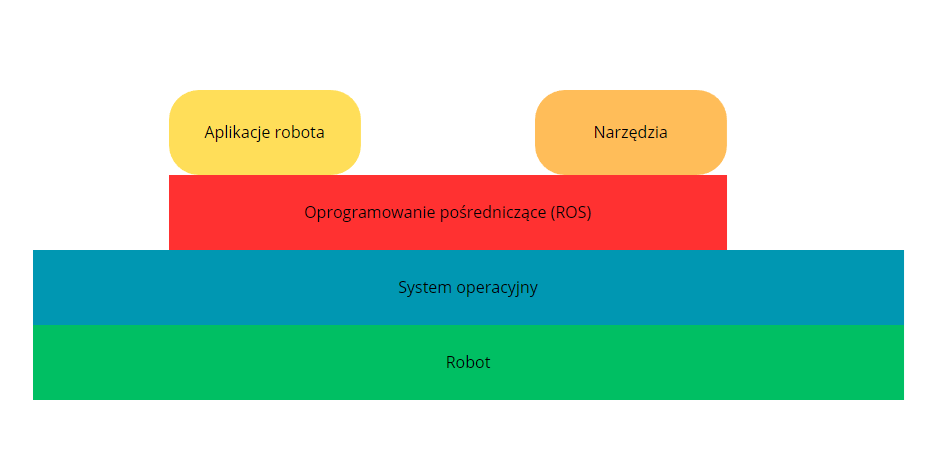
\includegraphics[width=0.8\textwidth]{images/middle.png}
	\caption{Reprezentacja pośrednika w systemie robota}
	\label{fig:middle}
	\end{figure}
\newline
Zasadniczo ROS 2 to otwartoźródłowe oprogramowanie bazujące na usłudze dystrybucji danych - DDS (ang. "Data Distribution Service"), które dostarcza ustandaryzowane narzędzia do organizacji kodu aplikacji w modularne pakiety, zapewniania współbieżnego wykonania kodu na wiele dostępnych plików wykonywalnych, oraz komunikację między tymi modułami podczas równoległego uruchomienia w systemie robota.\cite{bib:guide}

\newpage
\section{SLAM Toolbox}
SLAM Toolbox to zestaw narzędzi i rozwiązań do tworzenia map 2D w czasie rzeczywistym, stworzone przez Steve'a Mecenski.
 Stosowane algorytmy w przeszłości to np. GMapping, Karto, Cartographer oraz Hector, jednakże prawie żaden z nich nie potrafił tworzyć map w czasie rzeczywistym, jedynie Cartographer stworzony przez Google miał takie możliwości, lecz przestał być on wspierany.
 \cite{bib:slamtoolbox} Zastosowanie SLAM Toolbox pozwala na tworzenie map w czasie rzeczywistym obszarów, do nawet 24 000 m$^2$ przez niewykwalifikowanych użytkowników. Przykład działania SLAM Toolbox przedstawiono na rysunku poniżej.

\begin{figure}[h]
	\centering
	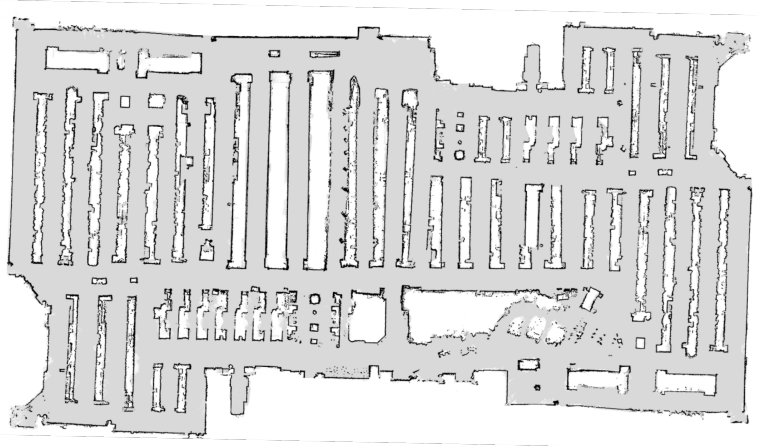
\includegraphics[width=0.8\textwidth]{images/sklep.png}
	\caption{Mapa sklepu utworzona za pomocą SLAM Toolbox}
	\label{fig:sklep}
	\end{figure}

SLAM Toolbox oferuje 3 główne tryby pracy:
\begin{itemize}
	\item \textbf{Mapowanie synchroniczne} - Ten tryb pozwala na mapowanie i lokalizację w przestrzeni zachowując dane poprzednich pomiarów. Pozwala to na większą dokładność mapy kosztem szybkości i odporności na przerwania.
	\item \textbf{Mapowanie asynchroniczne} - W tym trybie mapowanie i lokalizacja odbywają się wyłącznie na podstawie aktualnych pomiarów gdy ostatnie pomiary zakończą się i zostanie spełnione kryterium dokładności. Pozwala to na szybsze i mniej podatne na przerwania mapowanie kosztem jakości.
	\item \textbf{Lokalizacja} - W tym trybie robot dopasowuje aktualne pomiary do istniejącej mapy w celu określenia swojej pozycji. System tworzy tymczasowe punkty odniesienia z nowych pomiarów, które są używane do precyzyjnej lokalizacji. Po określonym czasie te tymczasowe punkty są usuwane, przywracając oryginalną mapę. Tryb ten może również działać bez wcześniejszej mapy, wykorzystując tylko lokalne pomiary do nawigacji.
\end{itemize}

\newpage
\subsection{Navigation2 (Nav2) i lokalizacja}
Nav2 jest to pakiet narzędzi do nawigacji robotów mobilnych w ROS 2. Zawiera on zestaw algorytmów do tworzenia modeli środowiska z sensorów, dynamicznego planowania ścieżki, obliczania prędkości silników i omijania przeszkód. 
Pakiet wykorzystuje drzewa zachowań (ang. "Behavior Trees") do definiowania zachowań robota, przez implementację wielu niezależnych zadań. Niektóre z nich odpowiadają za np. obliczanie trasy do celu, inne za naprawę błędów, a jeszcze inne za omijanie przeszkód. Dzięki komunikacji między tymi zadaniami, robot jest w stanie wykonywać skomplikowane zadania nawigacyjne.
\cite{bib:abs-2003-00368}
\newline
\newline
Do lokalizacji robota na mapie można wykorzystać wcześniej opisany SLAM Toolbox, jednak w pakiecie Nav2 dostępny jest również pakiet AMCL (ang. "Adaptive Monte Carlo Localization"), który pozwala na lokalizację robota na mapie z wykorzystaniem filtru cząsteczkowego. Algorytm ten polega na generowaniu losowych próbek (cząsteczek) reprezentujących możliwe położenia robota, a następnie porównywaniu ich z pomiarami z czujników. Cząsteczki, które najlepiej pasują do pomiarów są wybierane, a reszta jest odrzucana. W ten sposób algorytm estymuje pozycję robota na mapie. \cite{bib:amcl}
\subsection{ROS2 Control i sterowanie napędami}
ROS2 Control to platforma do sterowania, zarządzania i komunikacji pomiędzy urządzeniami w robotach z oprogramowaniem. \cite{bib:ros2control}. Dzięki takiemu rozwiązaniu można w łatwy sposób zarządzać silnikami, enkoderami, czy innymi urządzeniami w robocie. Dzięki temu można wykorzystać np. pakiet diffdrive\_arduino, do sterowania robotem z napędem różnicowym za pomocą Arduino. Pakiet ten pozwala również na sterowanie prędkością silników, odczyt enkoderów, obliczanie odometrii oraz transformację między układem odometrii a układem bazowym. \cite{bib:diffdrive}
 

\section{Wybór rozwiązań}
Na podstawie analizy dostępnych narzędzi, w projekcie zdecydowano się na wykorzystanie SLAM Toolbox do mapowania, AMCL do lokalizacji podczas nawigacji, Nav2 do planowania ścieżki i kontroli ruchu oraz ROS2 Control z DiffDrive Arduino do sterowania napędami. Wybór ten podyktowany jest stabilnością rozwiązań, oraz dobrą integracją komponentów w ekosystemie ROS 2 oraz aktywnym wsparciem społeczności i dostępnością dokumentacji.


%\begin{Definition}\label{def:1}
%Definicja to zdanie (lub układ zdań) odpowiadające na pytanie o strukturze „co to jest a?”. Definicja normalna jest zdaniem złożonym z 2 członów: definiowanego (łac. definiendum) i definiującego (łac. definiens), połączonych spójnikiem definicyjnym („jest to”, „to tyle, co” itp.). 
%\end{Definition}
%
%\begin{Theorem}[Pitagorasa]\label{t:pitagoras}
%W dowolnym trójkącie prostokątnym suma kwadratów długości przyprostokątnych jest równa kwadratowi długości przeciwprostokątnej tego trójkąta. 
%\end{Theorem}
%
%\begin{Example}[generalizacja]\label{ex:generalizacja}
%Przykładem generalizacji jest para: zwierzę i pies. Pies jest zwierzęciem. Pies jest uszczegółowieniem pojęcia zwierzę. Zwierzę jest uogólnieniem pojęcia pies.
%\end{Example}

%%%%%%%%%%%%%%%%%%%%%%%%




% TODO
\chapter{Wymagania i narzędzia}
\label{ch:wymagania-i-narzedzia}

W niniejszym rozdziale przedstawiono wymagania funkcjonalne systemu, przypadki użycia w formie diagramu UML, szczegółową specyfikację wykorzystanych komponentów sprzętowych oraz metodykę i etapy realizacji projektu.

\section{Wymagania funkcjonalne}
System powinien realizować następujące funkcje:
\begin{itemize}
\item Zdalne sterowanie robotem poprzez klawiaturę (teleop\_twist\_keyboard \cite{bib:teleop}) w celu eksploracji i mapowania otoczenia
\item Tworzenie i zapisywanie mapy otoczenia w czasie rzeczywistym 
\item Lokalizacja robota na zapisanej mapie z wykorzystaniem algorytmu AMCL
\item Autonomiczna nawigacja do wyznaczonych punktów na mapie z omijaniem przeszkód

\end{itemize}
\newpage
\section{Przypadki użycia}
Na rysunku \ref{fig:use-case} przedstawiono diagram przypadków użycia systemu. System umożliwia użytkownikowi zdalne sterowanie robotem, tworzenie mapy otoczenia, lokalizację robota na mapie oraz autonomiczną nawigację do wyznaczonych punktów. 
\begin{figure}[h]
\centering
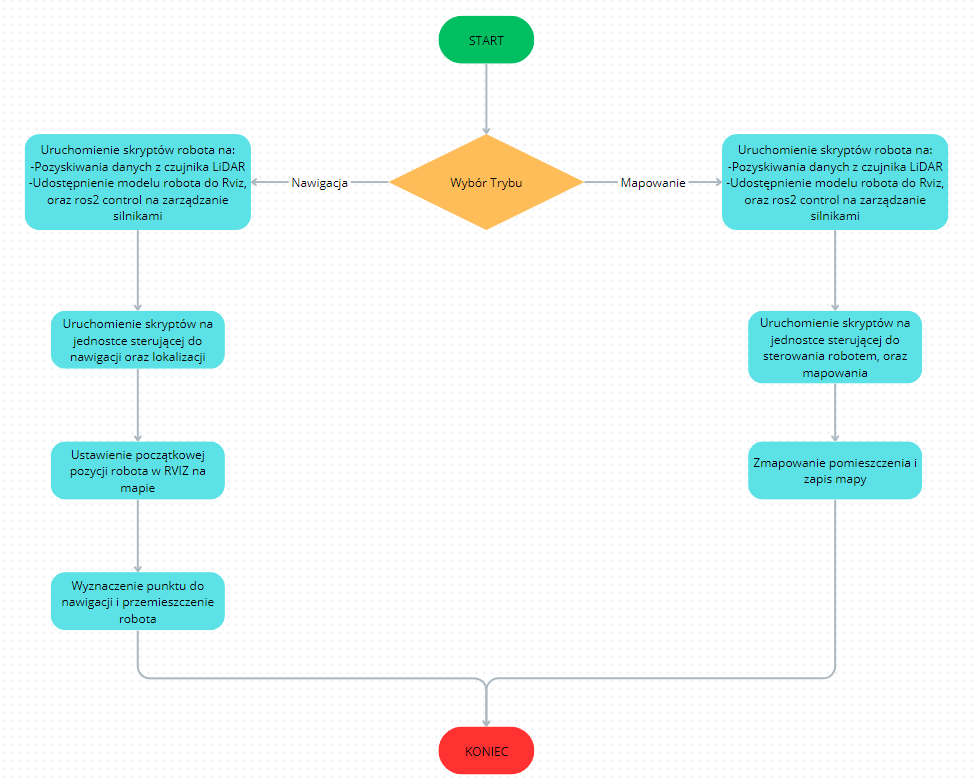
\includegraphics[width=0.8\textwidth]{images/UML.png}
\caption{Diagram przypadków użycia systemu}
\label{fig:use-case}
\end{figure}
\newpage
\section{Specyfikacja komponentów}
\subsection{Jednostki sterujące}
\begin{itemize}
\item Raspberry Pi 4 - główny komputer zarządzający robotem:
	\begin{itemize}
	\item System operacyjny Ubuntu 22.04
	\item ROS 2 Humble
	\item Komunikacja przez SSH z jednostką sterującą zachowaniem robota
	\end{itemize}
	\begin{figure}[h]
		\centering
		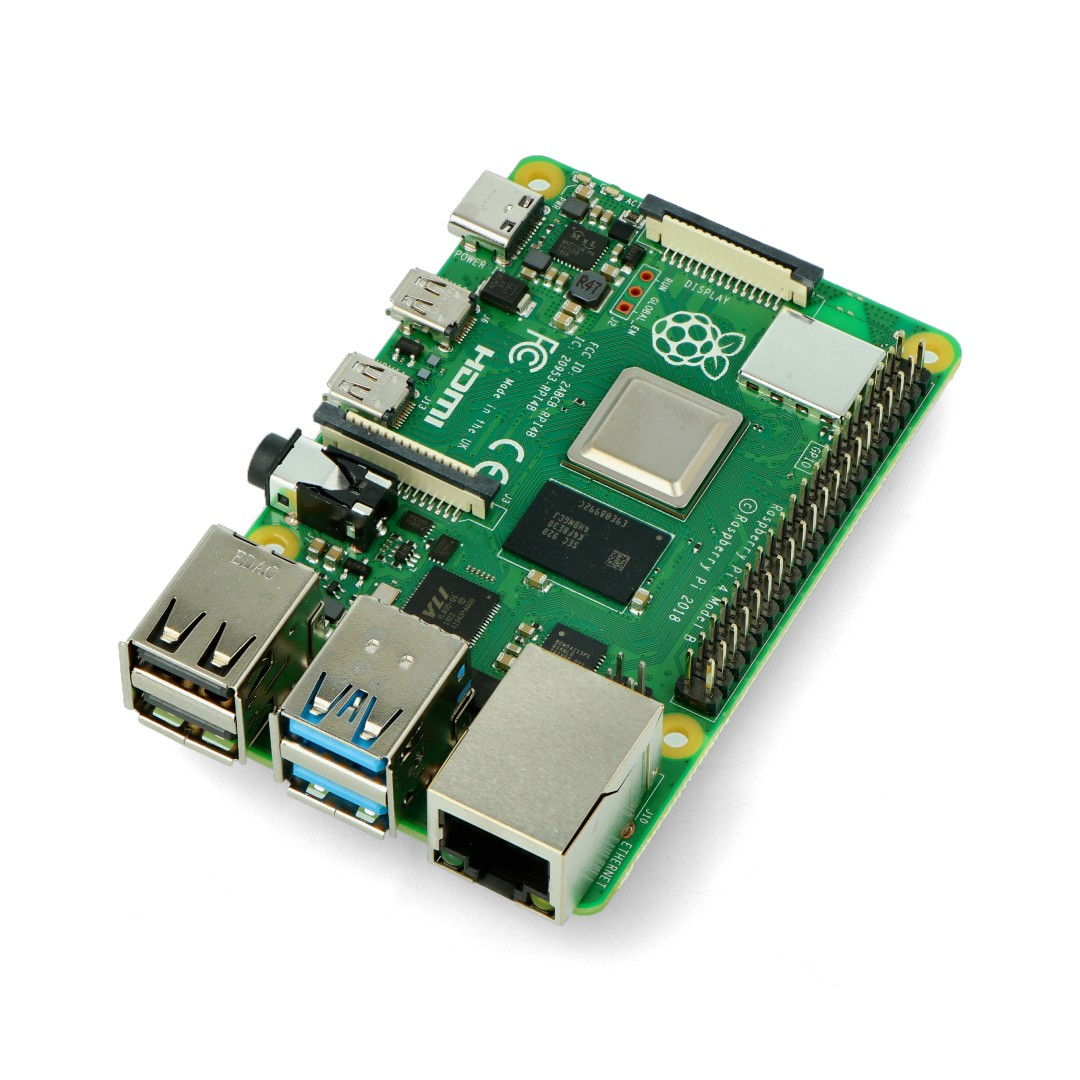
\includegraphics[width=0.4\textwidth]{images/rasp.png}
		\caption{Raspberry Pi 4 model B}
		\label{fig:raspberrypi4}
		\end{figure}
		\newpage	
		
\item Arduino Nano - sterownik silników:
	\begin{itemize}
	\item Obsługa enkoderów
	\item Komunikacja szeregowa z Raspberry Pi
	\end{itemize}

	\begin{figure}
		\centering
		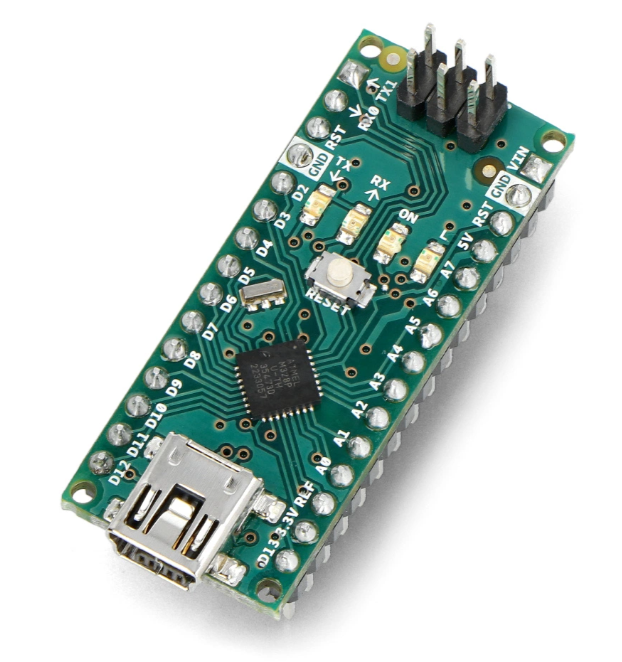
\includegraphics[width=0.4\textwidth]{images/nano.png}
		\caption{Arduino Nano}
		\label{fig:ardunano}
		\end{figure}
\end{itemize}

\subsection{Napęd}
\begin{itemize}
\item 2x silnik DC 12V 240RPM z metalową przekładnią
\item Wbudowane enkodery magnetyczne Halla
\begin{figure}
	\centering
	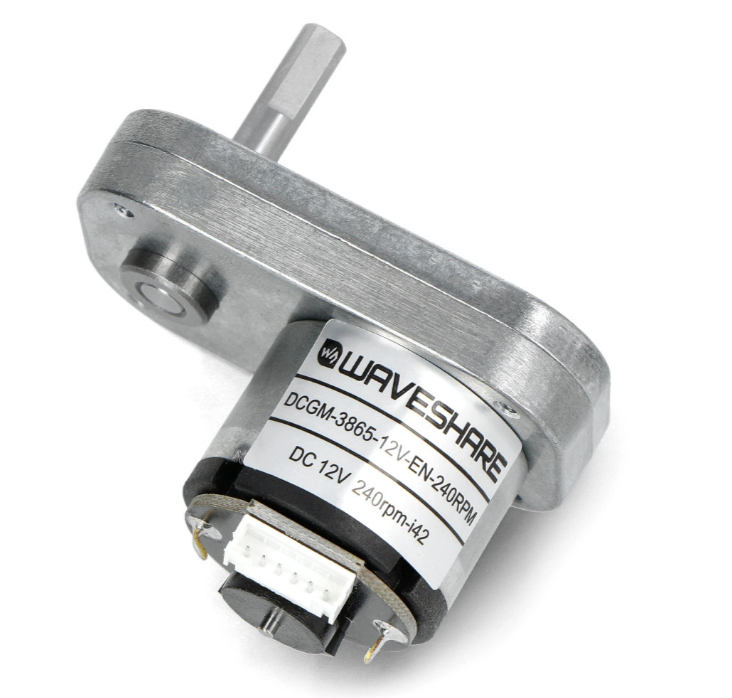
\includegraphics[width=0.4\textwidth]{images/sil.png}
	\caption{Silnik DC 12V 240RPM typu L z przekładnią metalową - magnetyczny enkoder Halla - Waveshare 22346}
	\label{fig:silnik}
	\end{figure}
\item Sterownik L298N - dwukanałowy mostek H \newline
\begin{figure}
	\centering
	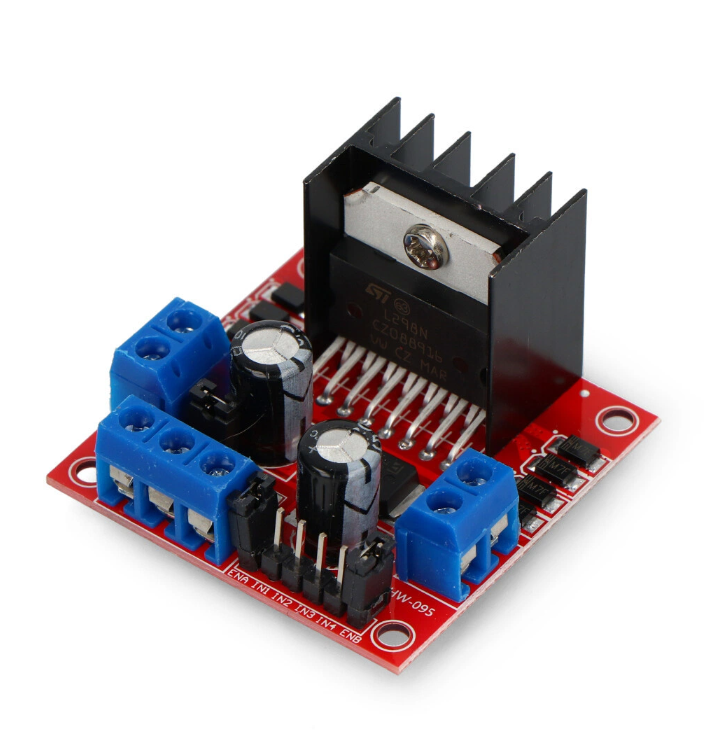
\includegraphics[width=0.4\textwidth]{images/ster.png}
	\caption{L298N - dwukanałowy sterownik silników - moduł 12V/2A}
	\label{fig:ster}
	\end{figure}
\end{itemize}


\subsection{Zasilanie}
\begin{itemize}
\item 6x akumulatory Li-ion 18650:
	\begin{itemize}
	\item 4 ogniwa (2S2P) dla silników
	\item 2 ogniwa (2S) dla elektroniki
	\end{itemize}
	\begin{figure}
		\centering
		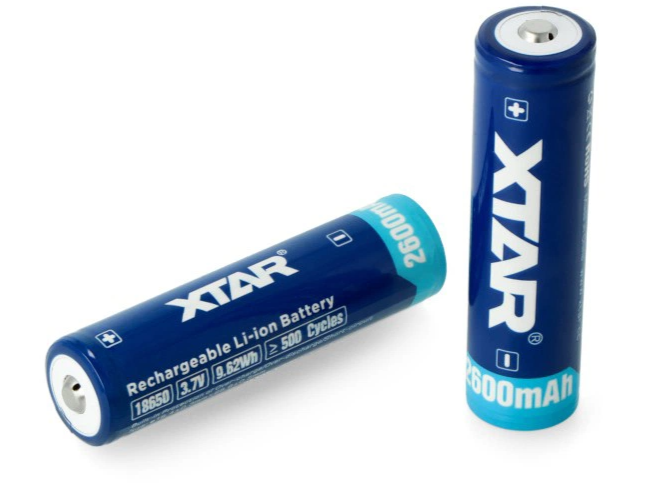
\includegraphics[width=0.4\textwidth]{images/ogniwo.png}
		\caption{Ogniwa 18650 Li-Ion XTAR - 2600mAh}
		\label{fig:ogniwa}
		\end{figure}
\item 2x przetwornica step-down:
	\begin{itemize}
	\item 12V dla silników
	\item 5V dla Raspberry Pi
	\end{itemize}
	\begin{figure}
		\centering
		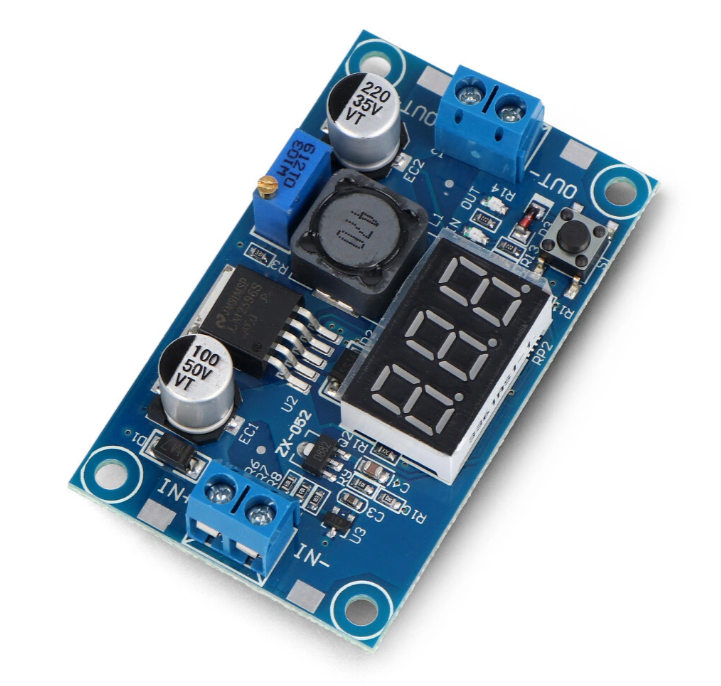
\includegraphics[width=0.4\textwidth]{images/przetwo.png}
		\caption{Przetwornica step-down LM2596 3,2V-35V 3A z wyświetlaczem}
		\label{fig:przetwo}
		\end{figure}
\end{itemize}
\newpage
\section{Sposób połączenia silników z Arduino i L298N}
\begin{figure}[h]
	\centering
	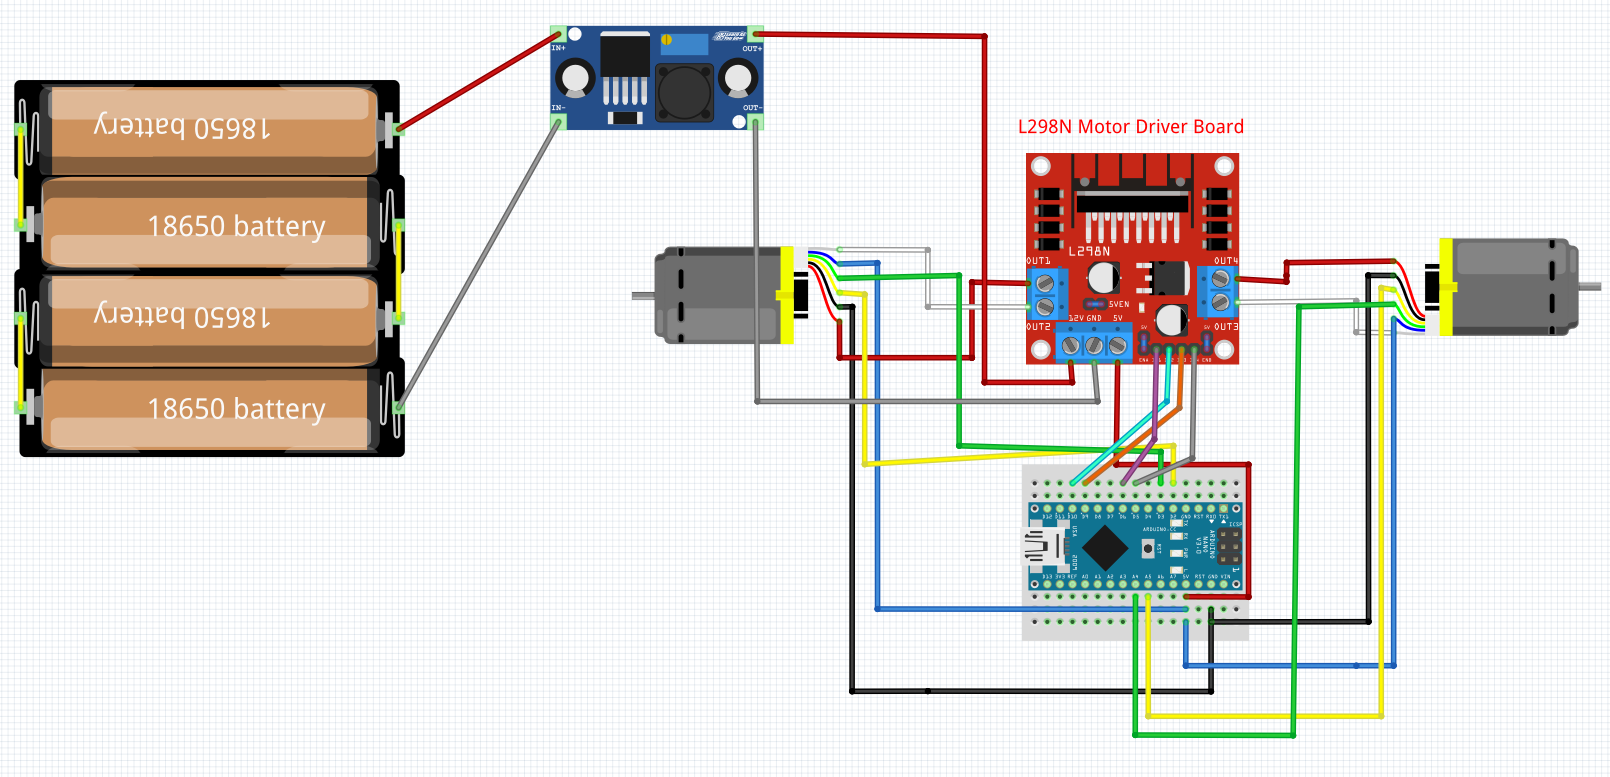
\includegraphics[width=0.9\textwidth]{images/schema_arduino.png}
	\caption{Schemat połączenia silników z Arduino i L298N}
	\label{fig:arduino-schema}
	\end{figure}
Na zaprezentowanym schemacie (rys. \ref{fig:arduino-schema}) przedstawiono sposób połączenia silników z Arduino i sterownikiem L298N. Silniki DC z enkoderami są zasilane z akumulatorów Li-ion, a sterowane przez Arduino Nano za pomocą sterownika L298N. Enkodery są podłączone do Arduino, które odczytuje impulsy i oblicza prędkość i położenie robota. Komunikacja między Arduino a Raspberry Pi odbywa się przez port szeregowy, co umożliwia przesyłanie danych o prędkości i położeniu robota.
\newpage

\section{Metodyka i etapy realizacji}
\subsection{Etap 1: Przygotowanie platformy sprzętowej}
\begin{itemize}
\item Instalacja systemu Ubuntu 22.04 na Raspberry Pi
\item Konfiguracja połączenia SSH
\item Instalacja ROS 2 Humble
\end{itemize}

\subsection{Etap 2: Implementacja sterowania napędem}
\begin{itemize}
\item Podłączenie silników do sterownika L298N
\item Programowanie Arduino - obsługa silników i enkoderów
\item Implementacja komunikacji szeregowej z Raspberry Pi
\end{itemize}

\subsection{Etap 3: Integracja sensorów}
\begin{itemize}
\item Montaż i konfiguracja LiDAR-a
\item Kalibracja czujników
\item Opracowanie układu mechanicznego i obudowy
\end{itemize}

\subsection{Etap 4: Implementacja oprogramowania}
\begin{itemize}
\item Konfiguracja pakietów ROS 2:
	\begin{itemize}
	\item SLAM Toolbox do mapowania
	\item Nav2 do nawigacji z AMCL do lokalizacji
	\item ROS2 Control do sterowania napędem
	\end{itemize}
\item Integracja i testy systemu
\end{itemize}



% TODO
\chapter{Specyfikacja użytkowa}
\label{ch:04}
W tym rozdziale przedstawiono wymagania użytkownika oraz specyfikację funkcjonalną systemu. Opisano kategorie użytkowników, sposób obsługi, administrację systemem, kwestie bezpieczeństwa oraz przykłady działania systemu.


\subsection{Wymagania sprzętowe i programowe}
Projekt ten stworzony był z myślą o następujących wymaganiach dla robota:
\newline
Sprzętowe:
\begin{itemize}
	\item Poruszać się w przestrzeni za pomocą sinlików, czyli np. przemieszczanie się do przodu, do tyłu, skręcanie w lewo i w prawo po korytarzach, czy w pomieszczeniach w równym podłożem.
	\item Skanować pomieszczenia za pomocą LiDAR-a, czyli zbieranie danych o otoczeniu wokół robota.
	\end{itemize}
Programowe:
\begin{itemize}
	\item Tworzyć mapę otoczenia, czyli zapisywanie danych z LiDAR-a w formie mapy 2D w czasie rzeczywistym i wizualizację tych danych w programie Rviz.
	\item Lokalizować się na mapie, czyli określanie pozycji robota na zapisanej mapie.
	\item Nawigować do wyznaczonych punktów, czyli planowanie trasy do punktów na mapie i omijanie przeszkód.
\end{itemize}
%\subsection{Metoda instalacji oprogramiwania i konfiguracji sprzętu}
%\begin{itemize}
%	\item Instalacja systemu Ubuntu 22.04 na Raspberry Pi
%	\item Konfiguracja połączenia SSH
%	\item Instalacja ROS 2 Humble na Raspberry Pi i komputerze sterującym
%	\item Podłączenie silników do sterownika L298N
%	\item Programowanie Arduino - obsługa silników i enkoderów
%	\item Implementacja komunikacji szeregowej z Raspberry Pi
%	\item Montaż i konfiguracja LiDAR-a
%	\item Kalibracja czujników
%	\item Opracowanie układu mechanicznego i obudowy
%	\item Konfiguracja pakietów ROS 2:
%	\begin{itemize}
%	\item SLAM Toolbox do mapowania
%	\item Nav2 do nawigacji z AMCL do lokalizacji
%	\item ROS2 Control do sterowania napędem
%	\end{itemize}
%\end{itemize}
\newpage
\subsection{Sposób aktywacji i korzystania z robota}
W tej sekcji wyjaśnione zostaną poszczególne etapy jakie należy podjąć do poprawnego uruchomienia i korzystania z robota.

Na samym początku należy uruchomić Raspberry Pi, przez włączenie zasilania, oraz załączenie silników.
Następnie należy przygotować terminale na jednostce sterującej (dwa terminale mają być połączone przez protokuł ssh z Raspberry Pi, a 5 terminali ma być przygotowanych na samej jednostce sterującej do uruchomienia późniejszych skryptów ROS). Przygotowanie tych terminali polega na odpowiednim:
\newline\newline
Dla jednostki sterującej: wejsciu do katalogu roboczego, uruchomienie komend source /opt/ros/humble/setup.bash, oraz source /install/setup.bash.
\newline\newline
Dla Raspberry Pi: wejsciu do katalogu roboczego, uruchomienie komend source /opt/ros/humble/setup.bash, oraz source /install/setup.bash.
\newline\newline
Następnie, należy uruchomić 2 skrypty przez ssh na Raspberry Pi, które odpowiadają za uruchomienie odpowiednich węzłów ROS. Pierwszy skrypt odpowiada za uruchomienie węzła odpowiedzialnego za sterowanie silnikami, a drugi za uruchomienie węzła odpowiedzialnego za odczyt danych z LiDAR-a. Odpowiednie komendy to: ros2 launch robot\_slam.launch.py oraz ros2 launch robot\_lidar.launch.py.
\newline\newline
Po uruchomieniu tych skryptów, należy uruchomić skrypt odpowiedzialny za sterowanie robotem za pomocą klawiatury. Komenda to: ros2 launch robot\_teleop.launch.py.
\newline\newline
Kolejnym krokiem jest uruchomienie skryptu odpowiedzialnego za mapowanie otoczenia. Komenda to: ros2 launch robot\_mapping.launch.py. W tym momencie gdy robot przemieszcza się przez komendy z klawiatury, pomieszczenie zostaje zmapowane.
\newline\newline
Gdy wystarczająco dużo pomieszczenia zostanie zmapowane, należy zapisać mapę. Można to wykonać przez komendę ros2 run nav2\_map\_server map\_saver -f map, lub przez dodanie panelu do Rviz z zestawu narzędzi SLAM Toolbox i zapisanie mapy z poziomu tego panelu.
\newline\newline
Z taką zapisaną mapą można zamknąć skrypty odpowiedzialne za sterowanie i mapowanie, jak i Rviz.
\newline\newline
Następnie, należy uruchomić skrypt odpowiedzialny za lokalizację robota na mapie, oraz skrypt odpowiedzialny za nawigację robota.\newline Komendy to: ros2 launch robot\_localization.launch.py,\newline ros2 launch robot\_navigation.launch.py. 
W wyniku uruchomienia tych skryptów powinien pojawić się nowy ekran Rviz, na którym będzie widoczna wcześniej zapisana mapa. Należy na niej umieścić robota przez wybranie z górnego zestawu narzędzi 2d-pose-estimate, a następnie kliknięcie na mapie w miejscu gdzie znajduje się robot. W tym momencie algorytm AMCL tworzy chmurę przewidywanych punktów w których może znajdować się robot. Następnie należy wybrać cel do którego robot ma się przemieścić, przez wybranie z górnego zestawu narzędzi 2d-nav-goal, a następnie kliknięcie na mapie w miejscu gdzie ma się znaleźć cel. Robot powinien samodzielnie przemieścić się do tego celu, omijając przeszkody.
\section{Administracja systemem}
System nie wymaga specjalnej administracji, jednakże w przypadku problemów z działaniem, można skorzystać z narzędzi diagnostycznych dostępnych w ROS 2, jak i z dokumentacji dostępnej na stronie internetowej ROS 2. W celu modyfikacji np. prędkością poruszania robota, przy korzystaniu z klawiatury, można zmienić prędkość przez naciśnięcie q i w. Do modyfikacji prędkości podczas nawigacji, można zmienić prędkość w pliku konfiguracyjnym Nav2.
\section{Kwestie bezpieczeństwa}
Robot opracowany został z myślą o omijaniu przeszkód, nawet tych których nie było na wcześniej stworzonej mapie pozwalając na bezpieczne poruszanie się w przestrzeni.
Należy jednak pamiętać że robot ten nie został przygotowany do pracy w środowiskach bez równego podłoża, dlatego należy unikać przemieszczania się po nierównym terenie co może prowadzić do przewrócenia się robota.
\section{Przykład działania i scenariusze korzystania z systemu}
Na poniższych obrazach zaprezentowano przykładowe działanie systemu na korytarzu uczelni. Na pierwszym obrazie  przedstawiono nawigację robota do wyznaczonego punktu.

Z mapy widać, że robot zmapował cały korytarz, a z nawigacji widać, że robot samodzielnie przemieszcza się do wyznaczonego punktu, omijając przeszkody.

Robot ten pozwala na mapowanie różnego rodzaju pomieszczeń, oraz na nawigację do wyznaczonych punktów, co pozwala na zastosowanie go w różnego rodzaju zastosowaniach, jak np. inspekcja pomieszczeń. Testy przeprowadzane były w małych pomieszczeniach nie przekraczających 40m, jednakże robot ten jest w stanie zmapować pomieszczenia nawet do 24 000m co wynika z dokumentacji Nav2 \cite{bib:abs-2003-00368}.
%%%%%%%%%%%%%%%%%%%%%
%% RYSUNEK Z PLIKU
%
%\begin{figure}
%\centering
%
\includegraphics[width=0.5\textwidth]{./politechnika_sl_logo_bw_pion_pl.pdf}
%\caption{Podpis rysunku zawsze pod rysunkiem.}
%\label{fig:etykieta-rysunku}
%\end{figure}
%Rys. \ref{fig:etykieta-rysunku} przestawia …
%%%%%%%%%%%%%%%%%%%%%
%
%%%%%%%%%%%%%%%%%%%%%
%% WIELE RYSUNKÓW 
%
%\begin{figure}
%\centering
%\begin{subfigure}{0.4\textwidth}
%    
\includegraphics[width=\textwidth]{./politechnika_sl_logo_bw_pion_pl.pdf}
%    \caption{Lewy górny rysunek.}
%    \label{fig:lewy-gorny}
%\end{subfigure}
%\hfill
%\begin{subfigure}{0.4\textwidth}
%    
\includegraphics[width=\textwidth]{./politechnika_sl_logo_bw_pion_pl.pdf}
%    \caption{Prawy górny rysunek.}
%    \label{fig:prawy-gorny}
%\end{subfigure}
%
%\begin{subfigure}{0.4\textwidth}
%    
\includegraphics[width=\textwidth]{./politechnika_sl_logo_bw_pion_pl.pdf}
%    \caption{Lewy dolny rysunek.}
%    \label{fig:lewy-dolny}
%\end{subfigure}
%\hfill
%\begin{subfigure}{0.4\textwidth}
%    
\includegraphics[width=\textwidth]{./politechnika_sl_logo_bw_pion_pl.pdf}
%    \caption{Prawy dolny rysunek.}
%    \label{fig:prawy-dolny}
%\end{subfigure}
%        
%\caption{Wspólny podpis kilku rysunków.}
%\label{fig:wiele-rysunkow}
%\end{figure}
%Rys. \ref{fig:wiele-rysunkow} przestawia wiele ważnych informacji, np. rys. \ref{fig:prawy-gorny} jest na prawo u góry.
%%%%%%%%%%%%%%%%%%%%%


%
%\begin{figure}
%\centering
%\begin{tikzpicture}
%\begin{axis}[
%    y tick label style={
%        /pgf/number format/.cd,
%            fixed,   % po zakomentowaniu os rzednych jest indeksowana wykladniczo
%            fixed zerofill, % 1.0 zamiast 1
%            precision=1,
%        /tikz/.cd
%    },
%    x tick label style={
%        /pgf/number format/.cd,
%            fixed,
%            fixed zerofill,
%            precision=2,
%        /tikz/.cd
%    }
%]
%\addplot [domain=0.0:0.1] {rnd};
%\end{axis} 
%\end{tikzpicture}
%\caption{Podpis rysunku po rysunkiem.}
%\label{fig:2}
%\end{figure}


% TODO
\chapter{Specyfikacja techniczna}
\label{ch:05}
Rozdział ten skupia się na aspektach technicznych projektu. Opisano w nim architekturę systemu, struktury danych, komponenty, moduły, biblioteki, algorytmy, wzorce projektowe, diagramy UML oraz szczegóły implementacji wybranych fragmentów.
\section{Idea robota autonomicznego mapującego w czasie rzeczywistym} 
Robot autonomiczny mapujący w czasie rzeczywistym to robot mobilny, który samodzielnie przemieszcza się w przestrzeni, zbierając dane o otoczeniu i tworząc mapę otoczenia w czasie rzeczywistym. Robot ten wykorzystuje różnego rodzaju sensory, jak np. LiDAR, kamery, czy enkodery, do zbierania danych o otoczeniu. Dane te są przetwarzane przez algorytmy SLAM (Simultaneous Localization and Mapping), które pozwalają na określenie pozycji robota na mapie oraz na tworzenie mapy otoczenia. Robot ten może być wykorzystywany w różnego rodzaju zastosowaniach, jak np. inspekcja pomieszczeń, czy przemieszczanie się w trudno dostępnych miejscach.
\section{Architektura systemu}
System składa się z kilku modułów, które współpracują ze sobą w celu zapewnienia poprawnego działania robota. Moduły te to:
\begin{itemize}
	\item Sterowanie silnikami - moduł odpowiedzialny za sterowanie silnikami robota
	\item Odczyt danych z LiDAR-a - moduł odpowiedzialny za odczyt danych z LiDAR-a
	\item Mapowanie - moduł odpowiedzialny za tworzenie mapy otoczenia
	\item Lokalizacja - moduł odpowiedzialny za lokalizację robota na mapie
	\item Nawigacja - moduł odpowiedzialny za nawigację robota
\end{itemize}
\section{Struktura systemu i objaśnienie działania algorytmów}
\subsection{Diagramy UML prezentujące działanie konkretnych programów}


% % % % % % % % % % % % % % % % % % % % % % % % % % % % % % % % % % % 
% Pakiet minted wymaga importu: \usepackage{minted}                 %
% i specjalnego kompilowania:                                       %
% pdflatex -shell-escape main                                       %
% % % % % % % % % % % % % % % % % % % % % % % % % % % % % % % % % % % 


Krótka wstawka kodu w linii tekstu jest możliwa, np.  \lstinline|int a;| (biblioteka \texttt{listings})% lub  \mintinline{C++}|int a;| (biblioteka \texttt{minted})
. 
Dłuższe fragmenty lepiej jest umieszczać jako rysunek, np. kod na rys \ref{fig:pseudokod:listings}% i rys. \ref{fig:pseudokod:minted}
, a naprawdę długie fragmenty – w załączniku.


\begin{figure}
\centering
\begin{lstlisting}
class test : public basic
{
    public:
      test (int a);
      friend std::ostream operator<<(std::ostream & s, 
                                     const test & t);
    protected:
      int _a;  
      
};
\end{lstlisting}
\caption{Pseudokod w \texttt{listings}.}
\label{fig:pseudokod:listings}
\end{figure}

%\begin{figure}
%\centering
%\begin{minted}[linenos,frame=lines]{c++}
%class test : public basic
%{
%    public:
%      test (int a);
%      friend std::ostream operator<<(std::ostream & s, 
%                                     const test & t);
%    protected:
%      int _a;  
%      
%};
%\end{minted}
%\caption{Pseudokod w \texttt{minted}.}
%\label{fig:pseudokod:minted}
%\end{figure}




% TODO
\chapter{Weryfikacja i walidacja}
\label{ch:06}
\begin{itemize}
\item sposób testowania w ramach pracy (np. odniesienie do modelu V)
\item organizacja eksperymentów
\item przypadki testowe zakres testowania (pełny/niepełny)
\item wykryte i usunięte błędy - problem z zasilaniem - filmik, problem z kolkami - funkcja w kodzie i jej objasnienie, problem z bledna nawigacją i przemieszczaniem sie mapy - obrazek i ze zle podlaczone silniki
\item opcjonalnie wyniki badań eksperymentalnych
\end{itemize}





% TODO
\chapter{Podsumowanie i wnioski}
\begin{itemize}
\item uzyskane wyniki w świetle postawionych celów i zdefiniowanych wyżej wymagań
\item kierunki ewentualnych danych prac (rozbudowa funkcjonalna …)
\item problemy napotkane w trakcie pracy
\end{itemize}



\backmatter

%\bibliographystyle{plplain}  % bibtex
%\bibliography{biblio} % bibtex
\addcontentsline{toc}{chapter}{Bibliografia}
\printbibliography
\begin{appendices}

% TODO
\chapter{Spis skrótów i symboli}

\begin{itemize}
\item[SLAM] jednoczesna lokalizacja i mapowanie (ang. \english{Simultaneous Localization and Mapping})
\item[LiDAR] urządzenie wykonujące wykrywanie światła i określanie odległości (ang. \english{Light Detection and Ranging})
\item[IMU] inercyjna jednostka pomiarowa (ang. \english{Inertial Measurement Unit})
\item[RGB-D] kamera rejestrująca obraz RGB oraz informację o głębi (ang. \english{RGB-Depth})
\item[Nav2] system nawigacji dla ROS 2 (ang. \english{Navigation 2})
\item[ROS] system operacyjny dla robotów (ang. \english{Robot Operating System})
\item[ROS2 Control] system kontroli robotów dla ROS 2 (ang. \english{Robot Operating System 2 Control})
\item[SLAM Toolbox] zestaw narzędzi do jednoczesnej lokalizacji i mapowania (ang. \english{Simultaneous Localization and Mapping Toolbox})
\end{itemize}


% TODO
\chapter{Źródła}

Jeżeli w pracy konieczne jest umieszczenie długich fragmentów kodu źródłowego, należy je przenieść w to miejsce.

\begin{lstlisting}
if (_nClusters < 1)
	throw std::string ("unknown number of clusters");
if (_nIterations < 1 and _epsilon < 0)
	throw std::string ("You should set a maximal number of iteration or minimal difference -- epsilon.");
if (_nIterations > 0 and _epsilon > 0)
	throw std::string ("Both number of iterations and minimal epsilon set -- you should set either number of iterations or minimal epsilon.");
\end{lstlisting}


% % % % % % % % % % % % % % % % % % % % % % % % % % % % % % % % % % % 
% Pakiet minted wymaga odkomentowania w pliku config/settings.tex   %
% importu pakietu minted: \usepackage{minted}                       %
% i specjalnego kompilowania:                                       %
% pdflatex -shell-escape praca                                      %
% % % % % % % % % % % % % % % % % % % % % % % % % % % % % % % % % % % 

%\begin{minted}[linenos,breaklines,frame=lines]{c++}
%if (_nClusters < 1)
%   throw std::string ("unknown number of clusters");
%if (_nIterations < 1 and _epsilon < 0)
%   throw std::string ("You should set a maximal number of iteration or minimal difference -- epsilon.");
%if (_nIterations > 0 and _epsilon > 0)
%   throw std::string ("Both number of iterations and minimal epsilon set -- you should set either number of iterations or minimal epsilon.");
%\end{minted}


% TODO
\chapter{Lista dodatkowych plików, uzupełniających tekst pracy} 


W systemie do pracy dołączono dodatkowe pliki zawierające:
\begin{itemize}
\item źródła programu,
\item dane testowe,
\item film pokazujący działanie opracowanego oprogramowania lub zaprojektowanego i~wykonanego urządzenia,
\item itp.
\end{itemize}


\listoffigures
\addcontentsline{toc}{chapter}{Spis rysunków}
\listoftables
\addcontentsline{toc}{chapter}{Spis tabel}

\end{appendices}

\end{document}


%% Finis coronat opus.

